\documentclass{article}

\usepackage{graphicx}
\usepackage{tikz}
\usepackage{tikzsymbols}
\usetikzlibrary{calc,patterns,shapes.geometric}
\pagestyle{empty}
\usepackage[margin=0pt]{geometry}
\geometry{papersize={14in,12in}}

\def\centerarc[#1](#2)(#3:#4:#5){\draw[#1] ($(#2)+({#5*cos(#3)},{#5*sin(#3)})$) arc (#3:#4:#5);}

\begin{document}
	\begin{figure}
		\centering
		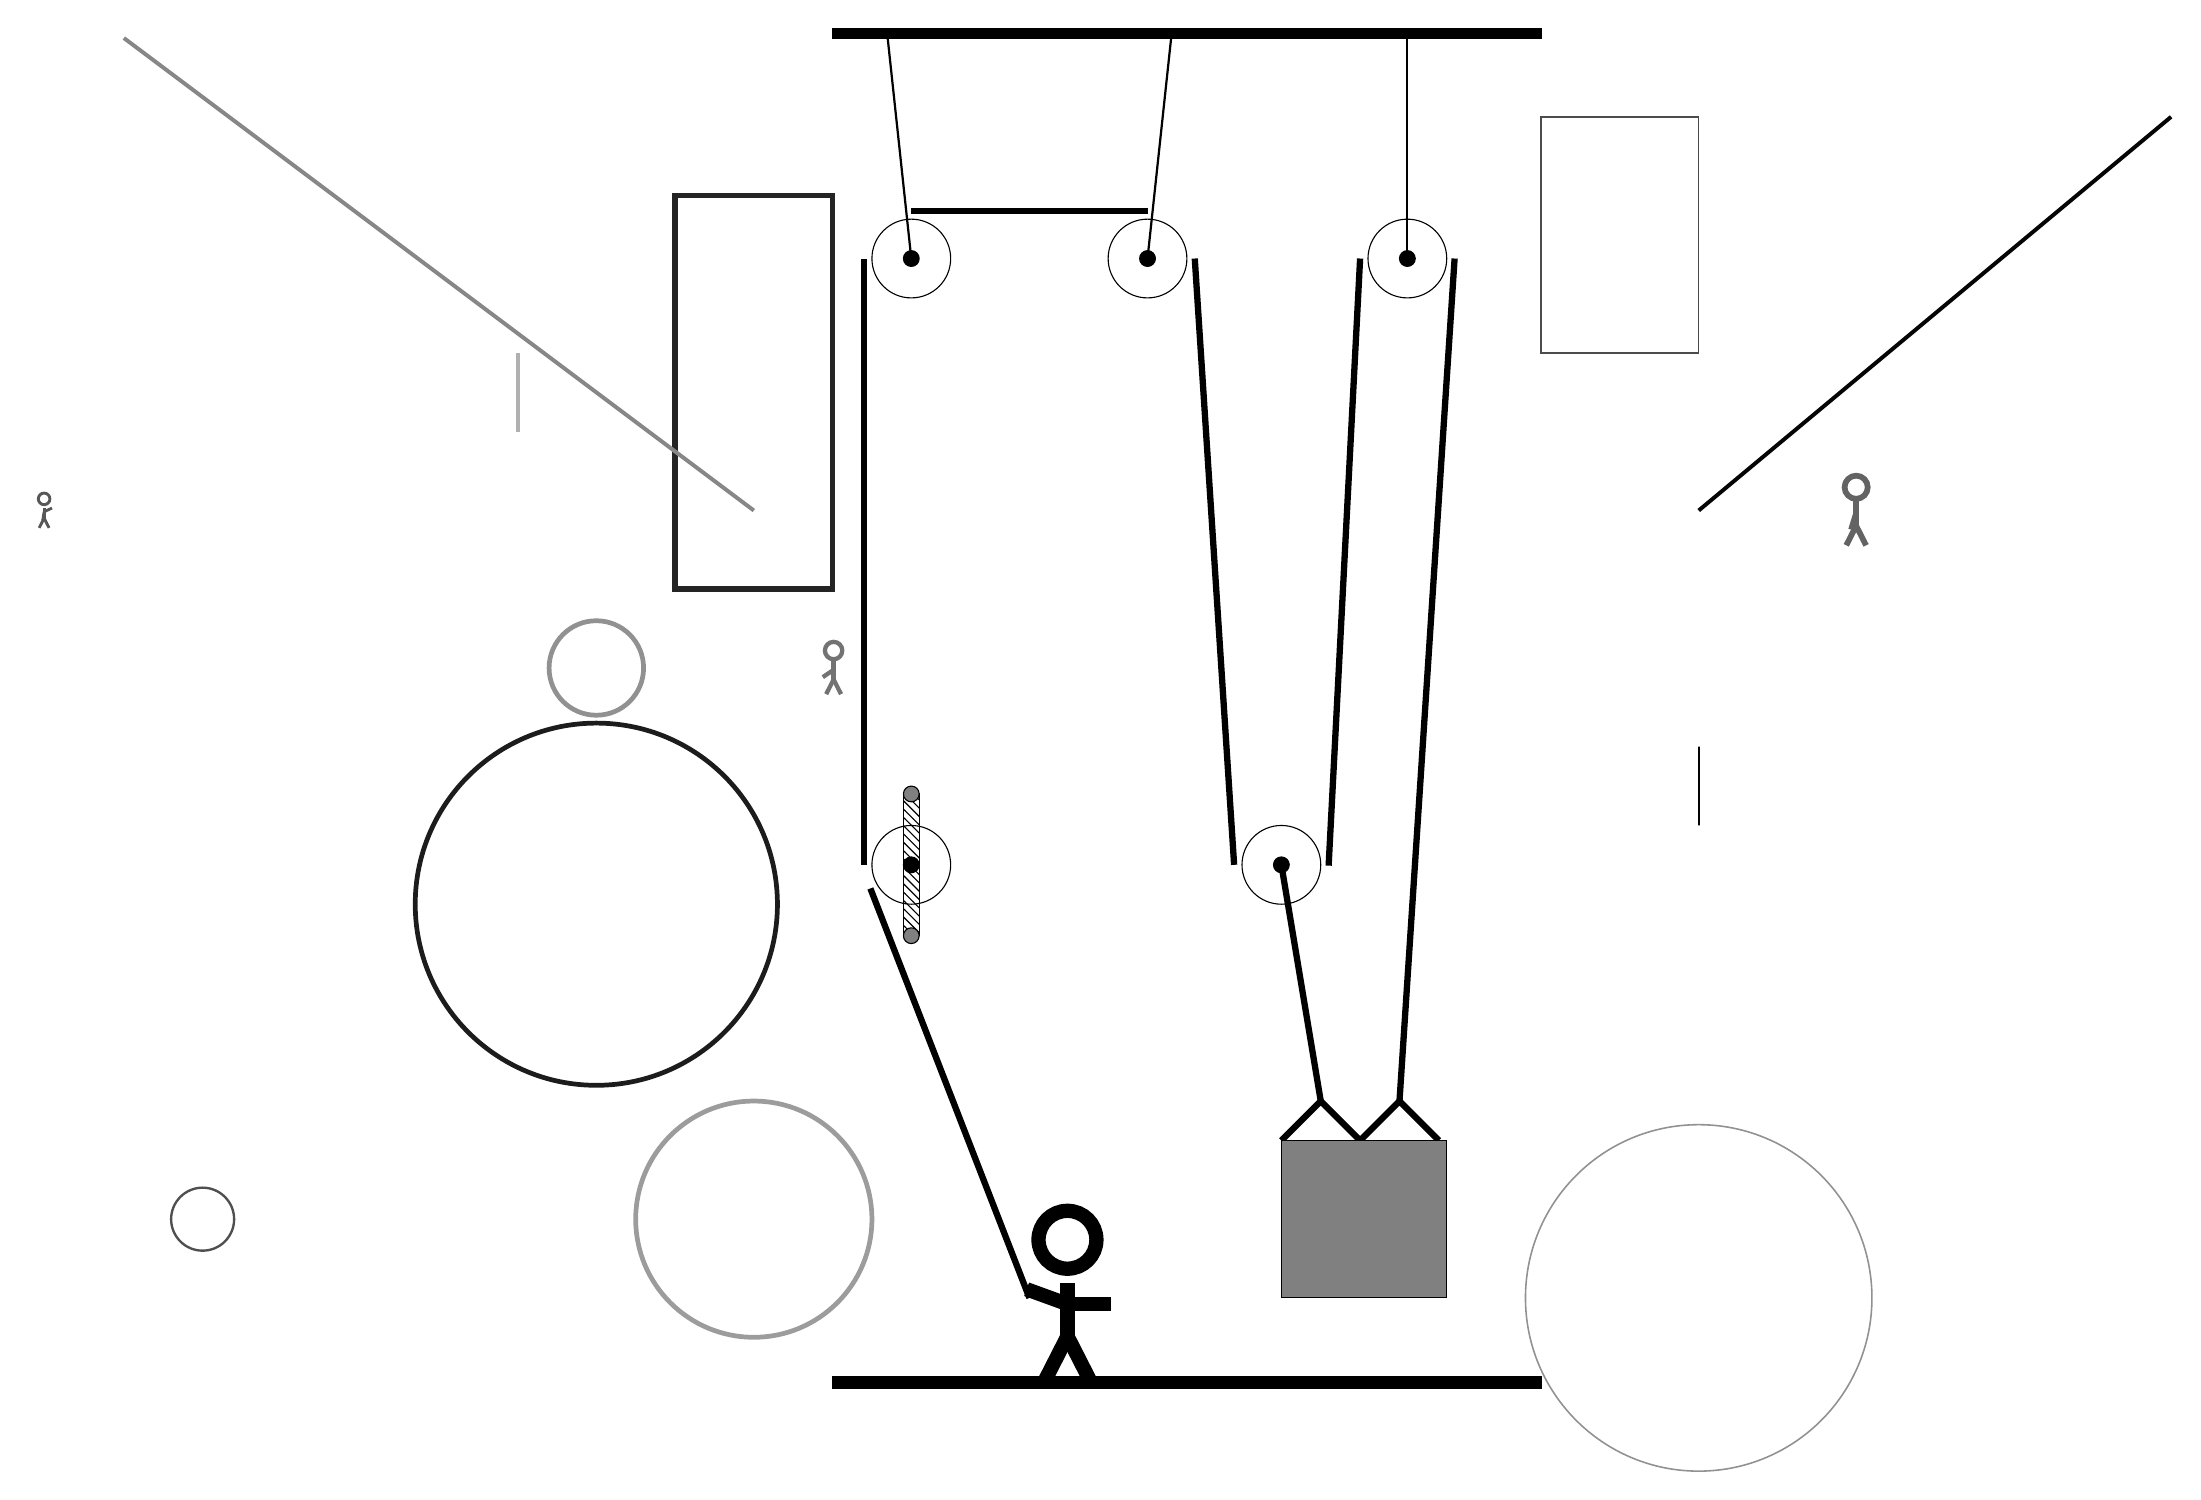
\begin{tikzpicture}
			%%%%% START %%%%%
			
			\draw[fill=black] (-3, 14) rectangle (6, 14.125);
			
			\draw (1, 11.2) circle (0.5);
			\draw[fill=black] (1, 11.2) circle (0.1);
			\draw[thick] (1, 11.2) -- (1.3, 14);
			
			\draw [line width=0.6mm, color=black!39](-4, -1) circle (1.5);
			
			\node[line width=0.2mm, color=black!66] at (-13, 8) {\Strichmaxerl[2][81][25]};
			\draw[line width=0.5mm, color=black!31](-7, 10) -- (-7, 9);
			\draw [line width=0.6mm, color=black!89](-6, 3) circle (2.3);
			\draw[line width=0.7mm, color=black!86] (-5, 12) rectangle (-3, 7);
			\draw[line width=0.5mm, color=black!98](8, 8) -- (14, 13);
			\node[line width=0.2mm, color=black!61] at (10, 8) {\Strichmaxerl[4][73][90]};
			\draw[line width=0.3mm, color=black!99] (8, 4) rectangle (8, 5);
			\node[line width=0.3mm, color=black!55] at (-3, 6) {\Strichmaxerl[3][34][90]};
			
			\draw[line width=0.2mm, color=black!70] (6, 13) rectangle (8, 10);
			\draw[line width=0.5mm, color=black!47](-4, 8) -- (-12, 14);
			\draw [line width=0.2mm, color=black!43](8, -2) circle (2.2);
			\draw [line width=0.6mm, color=black!43](-6, 6) circle (0.6);
			\draw [line width=0.3mm, color=black!69](-11, -1) circle (0.4);
			
			\draw (4.3, 11.2) circle (0.5);
			\draw[fill=black] (4.3, 11.2) circle (0.1);
			\draw[thick] (4.3, 11.2) -- (4.3, 14);
			
			\draw (2.7, 3.5) circle (0.5);
			\draw[fill=black] (2.7, 3.5) circle (0.1);
			
			\draw[line width=0.8mm]  (2.7, 0) -- (3.2, 0.5) -- (3.7, 0) -- (4.2, 0.5) -- (4.7, 0);
			\draw[fill=black!50] (2.7, 0) rectangle (4.8, -2);
			
			\draw (-2, 11.2) circle (0.5);
			\draw[fill=black] (-2, 11.2) circle (0.1);
			\draw[thick] (-2, 11.2) -- (-2.3, 14);
			
			\draw (-2, 3.5) circle (0.5);
			\draw[fill=black] (-2, 3.5) circle (0.1);
			\draw[pattern=north west lines, pattern color=black] (-2.1, 4.4) rectangle (-1.9, 2.6);
			\draw[fill=black!50] (-2, 4.4) circle (0.1);
			\draw[fill=black!50] (-2, 2.6) circle (0.1);
			
			\draw[line width=0.8mm](-0.5, -2) -- (-2.5196, 3.2);
			\centerarc[line width=0.8mm](-2, 3.5)(180:210:0.6);
			\draw[line width=0.8mm](-2.6, 3.5) -- (-2.6, 11.2);
			\centerarc[line width=0.8mm](-2, 11.2)(90:180:0.6);
			
			\draw[line width=0.8mm](-2, 11.8) -- (1, 11.8);
			\centerarc[line width=0.8mm](1, 11.2)(0:90:0.6);
			\draw[line width=0.8mm](1.6, 11.2) -- (2.1, 3.5);
			\centerarc[line width=0.8mm](2.7, 3.5)(180:370:0.6);
			\draw[line width=0.8mm] (3.3, 3.49) -- (3.7, 11.2);
			\centerarc[line width=0.8mm](4.3, 11.2)(0:180:0.6);
			\draw[line width=0.8mm](4.2, 0.5) -- (4.9, 11.2);
			\draw[line width=0.8mm] (3.2, 0.5) -- (2.7, 3.5);
			
			\node at (0, -2) {\Strichmaxerl[10][-20][0]};
			
			\draw[fill=black] (-3, -3) rectangle (6, -3.15);
			
			%%%%% END %%%%%
		\end{tikzpicture}
	\end{figure}	
\end{document}